\documentclass[tikz,convert={outfile=output.svg}]{standalone}
\usepackage{graphicx} % Required for inserting images
\usepackage{pgfplots}
\pgfplotsset{compat = newest}
\usepgfplotslibrary{colorbrewer}

\begin{document}

\pgfplotsset{ztick=\empty}
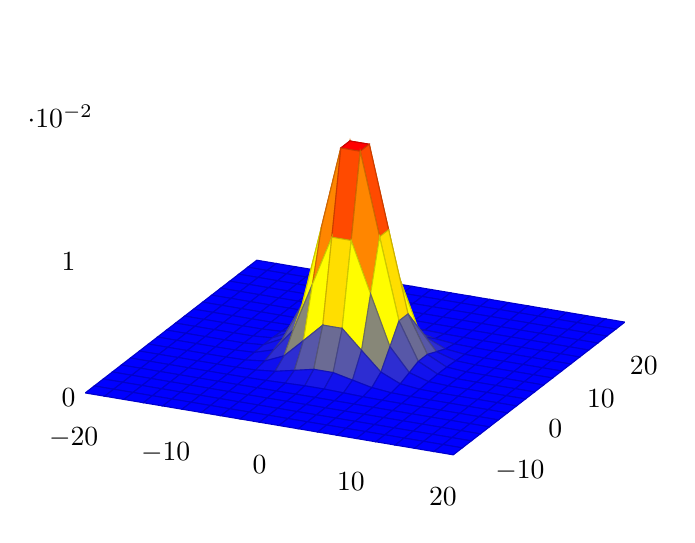
\begin{tikzpicture}
    \def\O{3}
    \begin{axis}[domain=-20:20, samples=20, axis line style={draw=none}, tick style={draw=none}, xtick={-20,-10,0,10,20}, ytick={-10,0,10,20}, xtick distance=5]
        \addplot3[surf] {(1/(2*pi*(\O)^2))*e^((-x^2 - y^2)/(2*(\O)^2};
    \end{axis}
\end{tikzpicture}

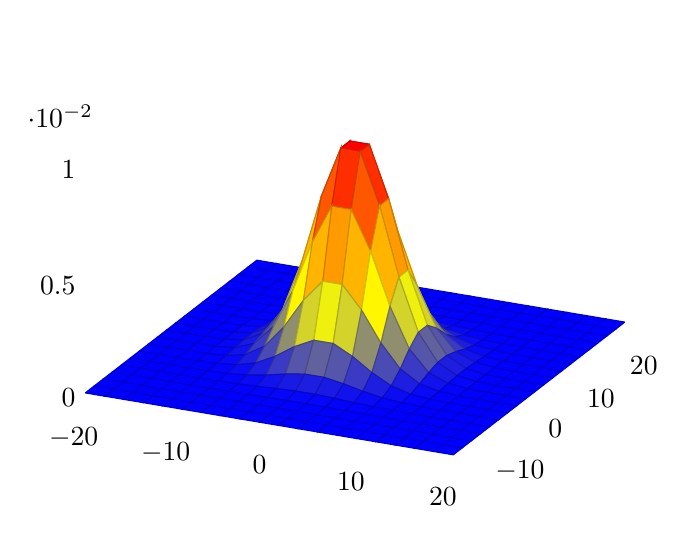
\begin{tikzpicture}
    \def\O{4}
    \begin{axis}[domain=-20:20, samples=20, axis line style={draw=none}, tick style={draw=none}, xtick={-20,-10,0,10,20}, ytick={-10,0,10,20}, xtick distance=5]
        \addplot3[surf] {(1/(2*pi*(\O)^2))*e^((-x^2 - y^2)/(2*(\O)^2};
    \end{axis}
\end{tikzpicture}

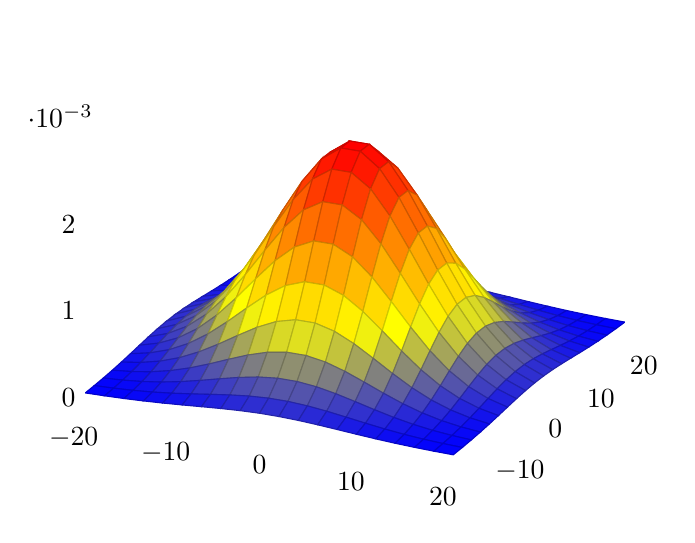
\begin{tikzpicture}
    \def\O{8}
    \begin{axis}[domain=-20:20, samples=20, axis line style={draw=none}, tick style={draw=none}, xtick={-20,-10,0,10,20}, ytick={-10,0,10,20}, xtick distance=5]
        \addplot3[surf] {(1/(2*pi*(\O)^2))*e^((-x^2 - y^2)/(2*(\O)^2};
    \end{axis}
\end{tikzpicture}

\end{document}